\documentclass[a4]{article}
\pagestyle{myheadings}

%%%%%%%%%%%%%%%%%%%
% Packages/Macros %
%%%%%%%%%%%%%%%%%%%
\usepackage{mathrsfs}


\usepackage{fancyhdr}
\pagestyle{fancy}
\lhead{}
\chead{}
\rhead{}
\lfoot{}
\cfoot{} 
\rfoot{\normalsize\thepage}
\renewcommand{\headrulewidth}{0pt}
\renewcommand{\footrulewidth}{0pt}
\newcommand{\RomanNumeralCaps}[1]
    {\MakeUppercase{\romannumeral #1}}

\usepackage{amssymb,latexsym}  % Standard packages
\usepackage[utf8]{inputenc}
\usepackage[russian]{babel}
\usepackage{MnSymbol}
\usepackage{mathrsfs}
\usepackage{amsmath,amsthm}
\usepackage{indentfirst}
\usepackage{graphicx}%,vmargin}
\usepackage{graphicx}
\graphicspath{{pictures/}} 
\usepackage{verbatim}
\usepackage{color}
\usepackage[nottoc,numbib]{tocbibind}
\usepackage{float}

\usepackage{listings}
\definecolor{codegreen}{rgb}{0,0.6,0}
\definecolor{codegray}{rgb}{0.5,0.5,0.5}
\definecolor{codepurple}{rgb}{0.58,0,0.82}
\definecolor{backcolour}{rgb}{0.95,0.95,0.92}
 
\lstdefinestyle{mystyle}{
    backgroundcolor=\color{backcolour},   
    commentstyle=\color{codegreen},
    keywordstyle=\color{magenta},
    numberstyle=\tiny\color{codegray},
    stringstyle=\color{codepurple},
    basicstyle=\footnotesize,
    breakatwhitespace=false,         
    breaklines=true,                 
    captionpos=b,                    
    keepspaces=true,                 
    numbers=left,                    
    numbersep=5pt,                  
    showspaces=false,                
    showstringspaces=false,
    showtabs=false,                  
    tabsize=2
}
 
\lstset{style=mystyle}

\usepackage{url}
\urldef\myurl\url{foo%.com}





\DeclareGraphicsExtensions{.pdf,.png,.jpg}% -- настройка картинок

\usepackage{epigraph} %%% to make inspirational quotes.
\usepackage[all]{xy} %for XyPic'a
\usepackage{color} 
\usepackage{amscd} %для коммутативных диграмм
%\usepackage[colorlinks,urlcolor=red]{hyperref}

%\renewcommand{\baselinestretch}{1.5}
%\sloppy
%\usepackage{listings}
%\lstset{numbers=left}
%\setmarginsrb{2cm}{1.5cm}{1cm}{1.5cm}{0pt}{0mm}{0pt}{13mm}


\newtheorem{Lemma}{Лемма}[section]
\newtheorem{Proposition}{Предложение}[section]
\newtheorem{Theorem}{Теорема}[section]
\newtheorem{Corollary}{Следствие}[section]
\newtheorem{Remark}{Замечание}[section]
\newtheorem{Definition}{Определение}[section]
\newtheorem{Designations}{Обозначение}[section]




%%%%%%%%%%%%%%%%%%%%%%% 
%Подготовка оглавления% 
%%%%%%%%%%%%%%%%%%%%%%% 
\usepackage[titles]{tocloft}
\renewcommand{\cftdotsep}{2} %частота точек
\renewcommand\cftsecleader{\cftdotfill{\cftdotsep}}
\renewcommand{\cfttoctitlefont}{\hspace{0.38\textwidth} \LARGE\bfseries} 
\renewcommand{\cftsecaftersnum}{.}
\renewcommand{\cftsubsecaftersnum}{.}
\renewcommand{\cftbeforetoctitleskip}{-1em} 
\renewcommand{\cftaftertoctitle}{\mbox{}\hfill \\ \mbox{}\hfill{\footnotesize Стр.}\vspace{-0.5em}} 
%\renewcommand{\cftchapfont}{\normalsize\bfseries \MakeUppercase{\chaptername} } 
%\renewcommand{\cftsecfont}{\hspace{1pt}} 
\renewcommand{\cftsubsecfont}{\hspace{1pt}} 
%\renewcommand{\cftbeforechapskip}{1em} 
\renewcommand{\cftparskip}{3mm} %определяет величину отступа в оглавлении
\setcounter{tocdepth}{5} 
\renewcommand{\listoffigures}{\begingroup %добавляем номер в список иллюстраций
\tocsection
\tocfile{\listfigurename}{lof}
\endgroup}
\renewcommand{\listoftables}{\begingroup %добавляем номер в список иллюстраций
\tocsection
\tocfile{\listtablename}{lot}
\endgroup}


   
   
%\renewcommand{\thelikesection}{(\roman{likesection})}
%%%%%%%%%%%
% Margins %
%%%%%%%%%%%
\addtolength{\textwidth}{0.7in}
\textheight=630pt
\addtolength{\evensidemargin}{-0.4in}
\addtolength{\oddsidemargin}{-0.4in}
\addtolength{\topmargin}{-0.4in}

%%%%%%%%%%%%%%%%%%%%%%%%%%%%%%%%%%%
%%%%%%Переопределение chapter%%%%%% 
%%%%%%%%%%%%%%%%%%%%%%%%%%%%%%%%%%%
\newcommand{\empline}{\mbox{}\newline} 
\newcommand{\likechapterheading}[1]{ 
\begin{center} 
\textbf{\MakeUppercase{#1}} 
\end{center} 
\empline} 

%%%%%%%Запиливание переопределённого chapter в оглавление%%%%%% 
\makeatletter 
\renewcommand{\@dotsep}{2} 
\newcommand{\l@likechapter}[2]{{\bfseries\@dottedtocline{0}{0pt}{0pt}{#1}{#2}}} 
\makeatother 
\newcommand{\likechapter}[1]{ 
\likechapterheading{#1} 
\addcontentsline{toc}{likechapter}{\MakeUppercase{#1}}} 




\usepackage{xcolor}
\usepackage{hyperref}
\definecolor{linkcolor}{HTML}{000000} % цвет ссылок
\definecolor{urlcolor}{HTML}{AA1622} % цвет гиперссылок
 
\hypersetup{pdfstartview=FitH,  linkcolor=linkcolor,urlcolor=urlcolor, colorlinks=true}

%%%%%%%%%%%%
% Document %
%%%%%%%%%%%%

%%%%%%%%%%%%%%%%%%%%%%%%%%%%%
%%%%%%главы -- section*%%%%%%
%%%%section -- subsection%%%%
%subsection -- subsubsection%
%%%%%%%%%%%%%%%%%%%%%%%%%%%%%
\def \newstr {\medskip \par \noindent} 



\begin{document}
\def\contentsname{\LARGE{Содержание}}
\thispagestyle{empty}
\begin{center} 
\vspace{2cm} 
{\Large \sc Санкт-Петербургский Политехнический}\\
\vspace{2mm}
{\Large \sc Университет} им. {\Large\sc Петра Великого}\\
\vspace{1cm}
{\large \sc Институт прикладной математики и механики\\ 
\vspace{0.5mm}
\textsc{}}\\ 
\vspace{0.5mm}
{\large\sc Кафедра прикладной математики}\\
\vspace{15mm}
%\rule[0.5ex]{\linewidth}{2pt}\vspace*{-\baselineskip}\vspace*{3.2pt} 
%\rule[0.5ex]{\linewidth}{1pt}\\[\baselineskip] 
{\huge \sc Лабораторная работа №$3$\\
\vspace{4mm}
Боксплот Тьюки
\vspace{6mm}
 }
\vspace*{2mm}
%\rule[0.7ex]{\linewidth}{1pt}\vspace*{-\baselineskip}\vspace{3.2pt} 
%\rule[0.5ex]{\linewidth}{2pt}\\ 
\vspace{1cm}

{\sc $3$ курс$,$ группа $3630102/70301$}

\vspace{2cm} 
Студент \hfill Лебедев К.С.\\
\vspace{1cm}
Преподаватель \hfill Баженов А. Н.\\
\vspace{20mm} 

\end{center} 
%\author{Я}
\begin{center}
\vfill {\large\textsc{Санкт-Петербург}}\\ 
2020 г.
\end{center}

%%%%%%%%%%%%%%%%%%%%%%%%%%%%%%%%%%%%%%%%%%%%%%%%%%%%%%%%%%%%%%%%%%%%%%%%%%%%%%%%%%%%%%%%%%%%%%
%\ \\[4cm]

%\rm
%%%%%%%%%%%%%%%%%%%%%%%%%%%%%%%%%%%%%%%%%%%%%%%%%%%%%%%%%%%%%%%%%%%%%%%%%%%%%%%%%%%%%%%%%%%%%%
\newpage
\pagestyle{plain}

%\begin{center}
%\begin{abstract} 

%\end{abstract}

%\end{center}

\newpage
\tableofcontents{}
\newpage
\listoffigures{}
\listoftables{}
\newpage

\section{Постановка задачи}

Для, приведённых ниже, пяти распределений сгенерировать выборки объёмом 20, 100, для каждой выборки построить боксплот Тьюки. Для каждого распределения определить процент выбросов экспериментально. Сгенерировать выборку, соответствующую распределению $1000$ раз и, вычислив средний процент, сравнить его с результатами, полученными теоретически.

Распределения:
\begin{itemize}
\item Стандартное нормальное распределение
\item Стандартное распределение Коши
\item Распределение Лапласа
\item Равномерное распределение 
\item Распределение Пуассона 
\end{itemize}


\section{Теория}

Боксплот Тьюки - график, использующийся в описательной статистике, изображающий одномерное распределение вероятностей.

Такой вид диаграммы в удобной форме показывает медиану, нижний и верхний квартили, минимальное и максимальное значение выборки и выбросы.

\begin{enumerate}
\item Выборочная медиана \cite{med}:
\begin{equation}
med\; x = \begin{cases}
x_{k+1}, & n = 2k+1\\
\frac{1}{2}\left(x_k+x_{k+1}\right), & n = 2k
\end{cases} \hfill  \label{eqn:med}
\end{equation}

\item Квартиль \cite{quart}:
\begin{equation}
z_{[p]} = \begin{cases}
x_{np}, & np \in \mathbb{Z}\\
x_{[np]+1}, & np \notin \mathbb{Z}
\end{cases} \hfill  \label{eqn:quart}
\end{equation}
\end{enumerate}

Выбросом в статистике называют результат измерения, выделяющийся из общей выборки.

\section{Реализация}
Для генерации выборки был использован $Python\;3.6$: модуль $random$ библиотеки $numpy$ \cite{numpy}.

Боксплот Тьюки был построен средствами библиотеки matplotlib \cite{plotlib}.

Правая и левые границы:  $R- LQ - l(UQ - LQ),\;L = UQ -k(UQ - LQ),$ где $k$ обычно полагают равным $1.5$ \cite{sas}

Число выбросов определялось таким образом: если значение из выборки находится вне установленных левой и правых границ, то оно является выбросом.




\newpage
\section{Результаты}
\begin{center}

\begin{figure}[H]
\caption{Boxplot нормальное распределение }
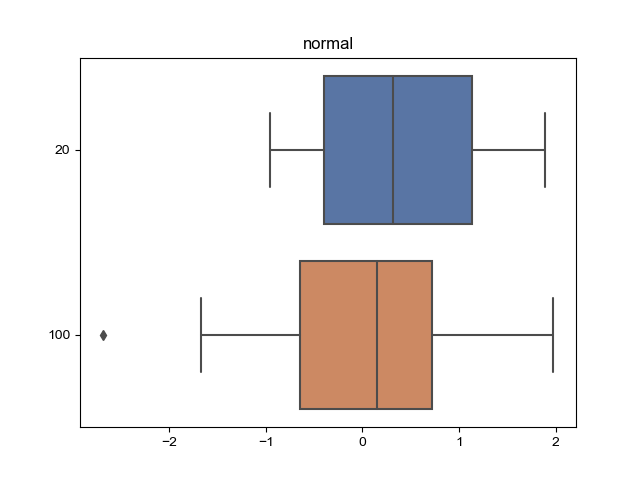
\includegraphics[width=\textwidth]{normal.png}
\end{figure}

\begin{figure}[H]
\caption{Boxplot стандартное распределение Лапласа }
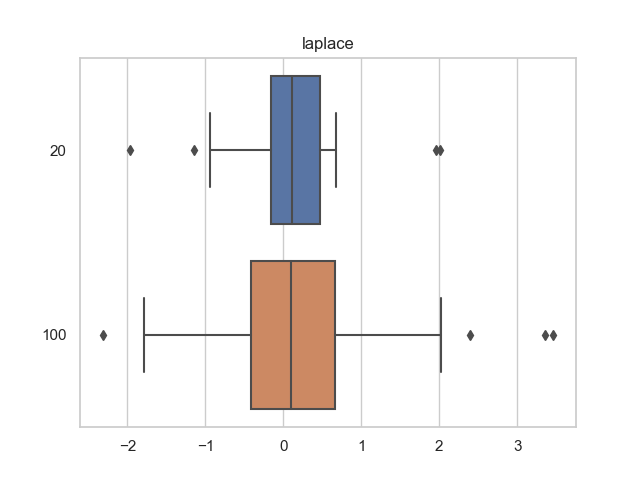
\includegraphics[width=\textwidth]{laplace.png} 
\end{figure}

\begin{figure}[H]
\caption{Boxplot стандартное распределение Коши }
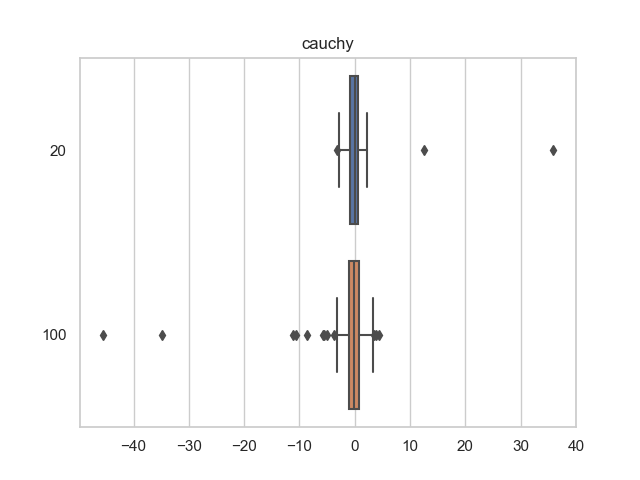
\includegraphics[width=\textwidth]{cauchy.png} 
\end{figure}

\begin{figure}[H]
\caption{Boxplot распределение Пуассона }
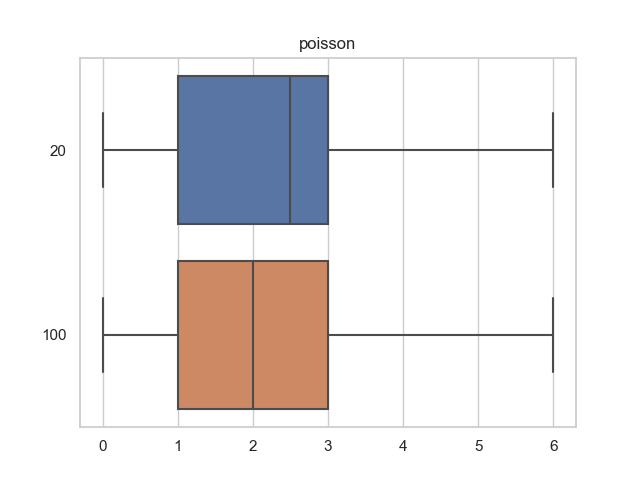
\includegraphics[width=\textwidth]{poisson.png} 
\end{figure}

\begin{figure}[H]
 \caption{Boxplot равномерное распределение }
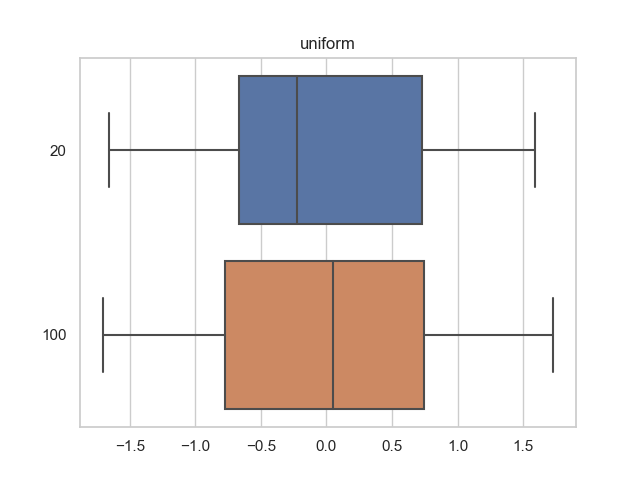
\includegraphics[width=\textwidth]{uniform.png}
\end{figure}

\begin{table}[H]
    
    \caption{Зависимость выбросов от размера выборки}
    \label{tab:my_label}
    \begin{center}
    \vspace{5mm}
    \begin{tabular}{|c|c|}
    \hline
    Выборка & Доля выбросов\\
    \hline
         normal	&\\
         \hline
n = 20   & 	0.022250 \\
\hline
n = 100   &	0.009710 \\
	\hline
cauchy	&\\
\hline
n = 20   & 	0.147700 \\
\hline
n = 100  & 	0.156480 \\
	\hline
laplace	&\\
\hline
n = 20    &	 0.072300 \\
\hline
n = 100   &	0.066380 \\
	\hline
uniform	&\\
\hline
n = 20    &	0.002200 \\
\hline
n = 100   &	0.000000 \\ 
	\hline
poisson	&\\
\hline
n = 20   & 	0.034300 \\
\hline
n = 100  & 	0.009650 \\
\hline
    \end{tabular}
    
    \end{center}
    
\end{table}

\end{center}


\section{Выводы}
\par Экспериментально полученные проценты выбросок, близки к теоретическим
Можно вывести соотношение между процентами выбросов:

\begin{equation}
uniform<normal<poisson<laplace<cauchy
\end{equation}

\par По полученным данным видно, что наименьший процент выбросов у равномерного распределения, а наибольший процент выбросов у распределения Коши

\begin{thebibliography}{}
    \bibitem{med}  
    Выборочная медиана  -  http://femto.com.ua/articles/part\_1/2194.html
    
    \bibitem{quart}  
    Квартили -  https://studfiles.net/preview/2438125/page:13/
    
    \bibitem{sas} 
    Боксплот - https://en.wikipedia.org/wiki/Box\_plot
    
    \bibitem{numpy}  
    Модуль numpy  -  https://physics.susu.ru/vorontsov/language/numpy.html
    
    \bibitem{plotlib} 
    Модуль matplotlib - https://matplotlib.org/users/index.html
    
 
\end{thebibliography}

\section{Приложения}


Код отчёта:\; \url{https://github.com/MisterProper9000/MatStatLabs/blob/master/MatStatLab3/MatStatLab3.tex}

Код лаборатрной:\; \url{https://github.com/MisterProper9000/MatStatLabs/blob/master/MatStatLab3/MatStatLab3.py}

\end{document}
